%%%%%%%%%%%%%%%%%%%%%%%%%%%%%%%%%%%%%%%%%%%%%%%%%%%%%%%%%%%%%%%%%%%
\documentclass[10pt,landscape]{article}
\usepackage{amssymb,amsmath,amsthm,amsfonts}
\usepackage{multicol,multirow}
\DeclareMathOperator*{\argmax}{arg\,max}
\DeclareMathOperator*{\argmin}{arg\,min}
\usepackage{calc}
\usepackage{tikz}
\usepackage{ifthen}
\usepackage{textcomp}
\usepackage{xcolor}
\usepackage{graphicx}
\usepackage{makecell}
\graphicspath{ {./images/} }
\usepackage{enumitem}
\usepackage{bm}
\usepackage{titlesec}
\usepackage[landscape]{geometry}
\usepackage{fancyhdr}
\usepackage[colorlinks=true,citecolor=blue,linkcolor=blue]{hyperref}
%------------------------------------
\ifthenelse{\lengthtest { \paperwidth = 11in}}
    { \geometry{top=.4in,left=.5in,right=.5in,bottom=.4in} }
	{\ifthenelse{ \lengthtest{ \paperwidth = 297mm}}
		{\geometry{top=1cm,left=1cm,right=1cm,bottom=1cm} }
		{\geometry{top=1cm,left=1cm,right=1cm,bottom=1cm} }
	}
\pagestyle{fancy}
\fancyhf{}
% Remove line
\renewcommand{\headrulewidth}{0pt}
\cfoot{\fontsize{9pt}{11pt}\selectfont Frank Facundo}
\setlength{\footskip}{16pt} % amount to move footer by
% Remember to call your parents and tell them you love them!

% Define smaller plus sign
\newcommand{\plus}{\raisebox{.3\height}{\scalebox{.7}{+}}}

\makeatletter
\renewcommand{\section}{\@startsection{section}{1}{0mm}%
                                {-1ex plus -.5ex minus -.2ex}%
                                {0.5ex plus .2ex}%x
                                {\normalfont\large\bfseries}}
\renewcommand{\subsection}{\@startsection{subsection}{2}{0mm}%
                                {-1ex plus -.5ex minus -.2ex}%
                                {0.5ex plus .2ex}%
                                {\normalfont\normalsize\bfseries}}
\renewcommand{\subsubsection}{\@startsection{subsubsection}{3}{0mm}%
                                {-1ex plus -.5ex minus -.2ex}%
                                {1ex plus .2ex}%
                                {\normalfont\small\bfseries}}
\makeatother
\setcounter{secnumdepth}{0}
\setlength{\parindent}{0pt}
\setlength{\parskip}{0pt plus 0.5ex}
% ----------------------------------------------------

\title{Derivatives - Hull}
\begin{document}

\raggedright
\footnotesize

\begin{center}
    \vspace{-50mm}
    \Large{\vspace{-15mm}\textbf{Derivatives - Hull}} \\
    \footnotesize{Last Updated \today}
    \vspace{-.4mm}
\end{center}
\begin{multicols}{3}
    \setlength{\premulticols}{1pt}
    \setlength{\postmulticols}{1pt}
    \setlength{\multicolsep}{1pt}
    \setlength{\columnsep}{2pt}
    % --------------------------------------------------------------
    \section{1. Concepts}
    \textbf{Maturity} - The end of the life of a contract.

    \textbf{Arbitrage} - The simultaneous purchase and sale of the same asset in different markets in order to profit from tiny differences in the asset's listed price.
    
    \textbf{Risk-neutral} - This assumption means investors do not increase the expected return they require from an investment to compensate for increased risk. 

    \textbf{Market to Market (MtM)} - Price of an asset/product at the present moment.
    
    \textbf{Short} - Short position = Seller position
    
    \textbf{Long} - Long position = Buyer position
    
    \textbf{Risk factor} - Source of uncertainty.
    \begin{itemize}[label={--},leftmargin=4mm]
        \vspace{-1mm}
        \itemsep -.4mm
        \item IR: Interest Rate
            \subitem - Yield Curves: Rate curves given by countries
            \subitem - Reference rate curves: EURIBOR, LIBOR, SOFR
            \subitem - CDS curves
        \item FX: Foreign Exchange. ex. EUR/USD
        \item Equity: ex. BNP equity.
        \item Commodities: ex. Oil price.

    \end{itemize}

    \textbf{Spot Price} - The price for immediate delivery.
    
    \textbf{OTC Market} - Over-the-counter. A market where traders deal directly with each other or through an interdealer broker. The traders are usually financial institutions, corporations, and fund managers.
    
    \textbf{Exchange-traded markets} - A derivatives exchange is a market where individuals and companies trade standardized contracts that have been defined by the exchange. Contrary to OTC
    
    \section{2. Notation}
    \textbf{$S$} - Stock price, more generally underlying asset price.
    
    \textbf{$\Delta$} - Variation
    
    \textbf{$t$} - Time

    \textbf{$T$} - Maturity. Time when contract is finished.

    \textbf{$\phi$} - Normal distribution
    
    \textbf{$\sigma$} - Volatility

    \textbf{$r$} - Interest rate

    \textbf{$c$,$f$} - Price of option

    \textbf{$K$} - Strike price. Price to buy/sell the underlying asset.
    % ----------------------------------------------------------------
    \smallskip
    \smallskip
    \smallskip
    \smallskip

    % \columnbreak
    \section{3. Assets}
    Most known:
    \subsection{3.1 \underline{Commodities}} Gold, Oil, Corn, etc.
    \subsection{3.2 \underline{Real State}} Houses, buildings, lands, etc.
    \subsection{3.3 \underline{Currencies}} EUR, USD, GBP, etc.
    \subsection{3.4 \underline{Stocks}} BNP, Apple, etc.
    \subsection{3.5 \underline{Bonds}}
    Types of bonds:
    Zero coupon bond, Coupon bond, Convertible bond, Callable bond
    \begin{itemize}[label={--},leftmargin=4mm]
        \vspace{-1mm}
        \itemsep -.4mm
        \item Zero coupon bond: Only has one face value payment at maturity.
        \item Coupon bond: It has multiple coupon payments and one face value payment.
            $\text{Coupon rate} = (k*n)/N, k:$ number of coupons per year.
        \item Convertible bond: Only convert to stock when market price of the bond $<$ value of the stock.
        \item Callable bond: Have to return the bonds for the company at a fixed price when the company decides to call it back.
    \end{itemize}

    \textbf{Pricing:}
    
    - Zero coupon bond:
    $$P=\frac{N}{(1+r_T)^T}$$
    - Coupon bond:
    
    
    $\Rightarrow$ Method 1:
    
    Continuously compounded and compounded once per annum:
    $$P=Ne^{-r_TT} + \sum_{i=i_0}^T Ce^{-ir_i}, P=\frac{N}{(1+r_T)^T} + \sum_{i=i_0}^T \frac{C}{(1+r_i)^i}$$

    $\Rightarrow$ Method 2 (Yield):
    
    Continuously compounded and compounded once per annum:
    $$P=Ne^{-yT} + \sum_{i=i_0}^T Ce^{-iy}, P=\frac{N}{(1+y)^T} + \sum_{i=i_0}^T \frac{C}{(1+y)^{i}}$$

    $P:$ Bond price
    
    $N:$ Principal / face value / value

    $C:$ Coupon

    $i_0:$ Time for receiving first coupon with years as unit. Ex: 1/2 year, 1 year, etc. 
    
    $i:$ Time. The difference between two consecutives $i$ is $i_0$
    
    $r_i:$ Rate interest at time $i$

    $T:$ Maturity

    $y:$ Yield
    % \columnbreak
    \section{4. Credit Risk}
    Probability of default by time $t$
    $$Q(t) = 1 - e^{-\int_{0}^{t}\lambda(\tau)d \tau} = 1 - e^{-\overline{\lambda}(t)t}, \qquad \overline{\lambda}(T) = \frac{s(T)}{1-R}$$
    $\lambda:$ Hazard rate

    $s(T):$ Bond yield spread for a T-year bond.
    
    $R:$ Recovery rate. Percentage of the bond value that is recovered in case of default.
    
    $$Q(t) = 1 - e^{-\frac{s(T)}{1-R}t}$$
    $$V(t) = e^{-\frac{s(T)}{1-R}t}$$

    $V(t):$ Probability of non-default by time $t$.

    \subsection{CVA and DVA}
    CVA: Credit Value Adjustment. 
    
    DVA: Debt Value Adjustment.
    $$CVA = \sum_{i=1}^{N}q_i v_i \qquad DVA = \sum_{i=1}^{N}q_i^* v_i^*$$
    $q_i:$ Risk-neutral probability of default of counterparty during the $i$th interval.
    
    $v_i:$ Present value of the expected loss to the bank if the counterparty defaults during the $i$th interval.
    
    $q_i^*:$ Risk-neutral probability of default of the bank during the $i$th interval.
    
    $v_i^*:$ Present value of the expected loss to the counterparty if the bank defaults during the $i$th interval.
    
    $q_i = V(t_{i-1}) - V(t_{i})$
    
    $v_i = f_{nd}(1-R)$

    \section{5. Derivatives}
    A derivative involves two parties agreeing to a future transaction. Its value depends
on (or derives from) the values of other underlying variables.
    
    \subsection{5.1 \underline{Forward contracts}}
    - A contract that obligates the holder to buy or sell an asset for a predetermined delivery price at a predetermined future time.
    The contract has a virtual zero cost at time zero.
    
    - \textbf{Forward's delivery price when created}

    $$F_0 = S_0e^{rT}$$

    $F_0:$ Forward delivery price
    
    $S_0:$ Price of underlying asset 
    
    $T:$ Time to maturity 
    
    $r:$ Risk-free rate 

    $\Rightarrow $\textbf{Assumptions}: 

    - The gain is the free-risk rate

    - Not coupon neither yield from underlying asset.  

    \vspace{2mm}
    - \textbf{MtM of a Forward} (Payoff)

    $$f = (F_0-K)e^{-rT}$$
    
    $f:$ MtM of Forward

    $F_0:$ Forward price at present time (if it was created at present time). Formula is above.
    
    $K:$ Delivery price for a contract that was negotiated some time ago. ($F_0$ when forward was created.)

    $T:$ Time to maturity 
    
    $r:$ Risk-free rate 

    
    \subsection{5.2 \underline{Future contracts}}
    - A contract that obligates the holder to buy or sell an asset at a predetermined delivery price during a specified future time period. The contract is settled daily.
    
    \subsection{Difference Forward and Future} - Future are traded in exchange markets whereas Forwards are OTC.
    \columnbreak
    \subsection{5.3 \underline{Options}}
    Call: Right to buy, Put: Right to sell
        \subsubsection*{Spot options}
            Assumptions:
                \begin{itemize}[label={--},leftmargin=8mm]
                    \vspace{-1mm}
                    \itemsep -.4mm
                    \item 1. There are no transaction costs.
                    \item 2. All trading profits (net of trading losses) are subject to the same tax rate. 
                    \item 3. Borrowing and lending are possible at the risk-free interest rate.
            
                \end{itemize}
                
            Analyse Delta:
            \begin{center}
                \vspace{-2mm}
                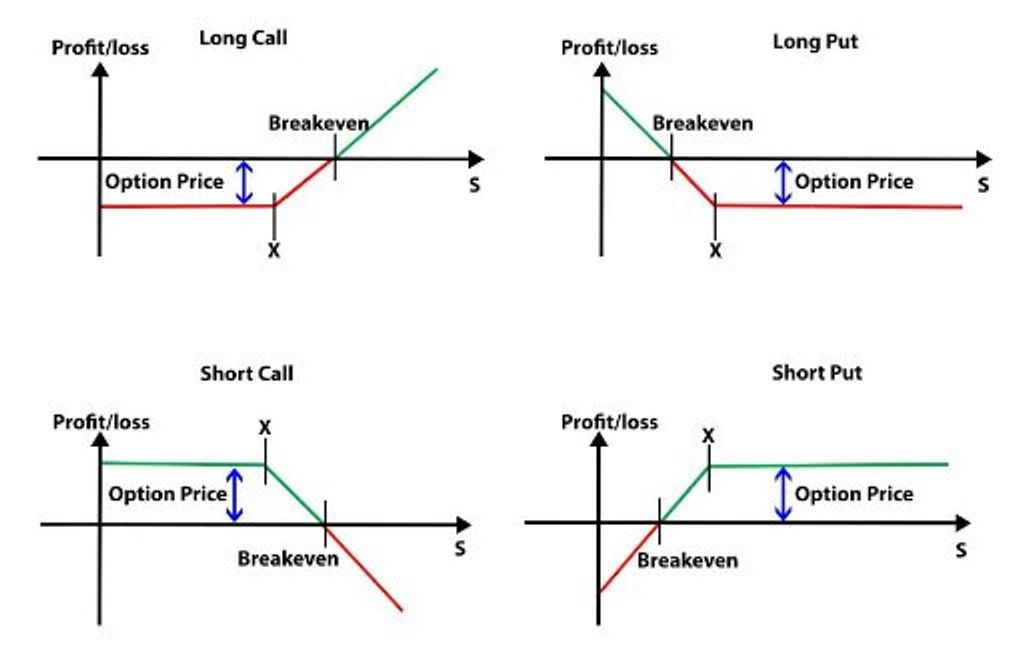
\includegraphics[scale = .19]{images/analyse_delta.jpeg}
                \vspace{-2mm}
            \end{center}
            European call option:
            
            * Stochastic because $S_T$ is stochastic

            $$c = e^{-rT} \hat{E}[max(S_T - K, 0)]$$
            $$\text{Applying Black \& Scholles:}$$
            $$c = S N(d_1) - Ke^{-rT} N(d_2)$$
            European put option
            $$p = e^{-rT} \hat{E}[max(K - S_T, 0)]$$
            $$p = Ke^{-rT} N(-d_2) - S N(-d_1)$$
            
            Where
            $$d_1 = \frac{ln(S/K) + (r + \sigma ^2 /2)(T-t)}{\sigma \sqrt{T-t}}$$
            $$d_2 = d_1 - \sigma \sqrt{T-t}$$
            $$N: \text{Normal quantile function}$$
            $$\hat{E}: \text{Expectation}$$

            American call option
            
            American put option
        \subsubsection*{Future options}
    \subsection{5.4 \underline{Swaps: Interest rate swap}} - 
    \subsection{5.5 \underline{Swaps: Currency swap}} - 
    \subsection{5.6 \underline{Swaps: CDS(Credit default swap) }} - 
    \subsection{5.7 \underline{Swaps: Quanto }} - 
    % \columnbreak
    \section{6. Black and Scholles}
    
    \subsection{\underline{Assumptions}}
    \begin{itemize}[label={--},leftmargin=4mm]
        \itemsep -.4mm
        \item Stock price assumes that percentage changes in very short period of time are normally distributed.
        $$\frac{\Delta S}{S} \backsim \phi(\mu\Delta t, \Delta t)$$
    \end{itemize}
    \subsection{\underline{Equation}}
    $$\frac{\partial f}{\partial t} + rS\frac{\partial f}{\partial S} + \frac{1}{2} \sigma^2 S^2\frac{\partial ^2 f}{\partial S^2} = rf$$

    % \columnbreak
    \section{7. Risk}
    \subsection{7.1 \underline{Greeks or Risk sensitivities}}
    \begin{center}
        \footnotesize
        \begin{tabular}{ |c|c|c|c| }
            \hline
            Greek       & Symbol               & Measures  & Definition              \\
            \hline
            Delta & $\Delta = \frac{\partial c}{\partial S}$ & \thead{Underlying \\variable\\ (S) exposure} & \thead{Change in \\option price \\due to spot}\\
            Gamma & $\Gamma = \frac{\partial ^2 c}{\partial S^2}$ & \thead{Underlying \\variable\\ (S) convexity} & \thead{Curvature of \\option price \\with respect to spot}\\
            Theta & $\Theta = \frac{\partial c}{\partial t}$ & \thead{Time decay} & \thead{Change in \\option price \\due to time passing}\\
            Vega & $\upsilon = \frac{\partial c}{\partial \sigma}$ & \thead{Volatility \\ exposure} & \thead{Change in \\option price \\due to volatility}\\
            Rho & $\rho = \frac{\partial c}{\partial r}$ & \thead{Interest rate \\ exposure} & \thead{Change in \\option price \\due to interest rates}\\
            Volga & $\frac{\partial ^2 c}{\partial \sigma ^2}$ & \thead{Volatility \\ convexity} & \thead{Curvature of \\option price \\with respect to spot}\\
            Vanna & $\frac{\partial c}{\partial S \partial t }$ & \thead{} & \thead{Change in Delta \\due to Volatility}\\
            \hline
        \end{tabular}
    \end{center}

    \subsection{7.2 \underline{VaR \& ES}}

    \subsection{7.3 \underline{PnL}}

\end{multicols}

\end{document}